\chapter{Caracterización y clasificación del comportamiento}\label{cha:mapa}

Con el objetivo de comprender cómo se modifica el comportamiento animal durante el aprendizaje de una nueva habilidad, decidimos comenzar estudiando el patrón de movimientos de ratones previamente entrenados en la tarea \textit{rotarod} con aceleración. Para ello clasificaremos, de manera no supervisada, diferentes tipos de poses que los ratones adoptan durante la ejecución de la tarea con el objetivo final de cuantificar el comportamiento animal de manera reproducible y automatizada.

A continuación explicaremos el procedimiento llevado a cabo para la clasificación del comportamiento animal. Primero, en la Sección \ref{sec:protocolo} describiremos el protocolo experimental de entrenamiento al cual fueron sometidos los ratones. Es importante aclarar que una vez que los ratones fueron entrenados en la tarea \textit{rotarod}, se registraron videos de la actividad de los mismos durante la ejecución de la tarea aprendida. Luego de la descripción del protocolo experimental, detallaremos en la Sección \ref{sec:videos} el proceso de análisis de los videos de los ratones, con el fin de extraer las posiciones de algunas partes de sus cuerpos en función del tiempo. Después, en la Sección \ref{sec:tsne} explicaremos cómo se clasificaron estos conjuntos de datos de posiciones utilizando un algoritmo de reducción de la dimensión llamado t-SNE. Utilizando el algoritmo t-SNE obtendremos un mapa bidimensional de comportamientos de los ratones. Finalmente, en la Sección \ref{sec:watershed} introduciremos el método utilizado para identificar y segmentar \textit{clusters} en este mapa de comportamientos.

\section{Protocolo experimental}\label{sec:protocolo}

En primera medida, es importante introducir el protocolo de entrenamiento de los ratones que se siguió en esta parte del trabajo. Este protocolo puede dividirse esencialmente en dos partes, habituación y entrenamiento, y tiene una duración total de entre 7 a 8 días.
\begin{enumerate}
\item Habituación (días 1 y 2): antes de dar inicio a las sesiones de entrenamiento (pruebas o \textit{trials}), los animales son habituados al experimentador y al ambiente del experimento (es decir, a la sala donde se encuentra el rotarod y al aparato \textit{rotarod} en sí). Esta etapa comprende los dos primeros días del protocolo, en los cuales los ratones son trasladados a la sala de experimentación y expuestos al \textit{rotarod}, fuera de funcionamiento, durante 10 a 15 minutos.

\item Entrenamiento (día 3 en adelante): cada día de entrenamiento consiste en 4 pruebas sucesivas de \textit{rotarod}, separadas entre sí por 5 minutos de descanso. En cada prueba el animal es colocado sobre el cilindro del \textit{rotarod}, que gira a velocidades crecientes con aceleración constante, desde 5 rpm hasta 45 rpm en 5 minutos, o hasta que el ratón se cae (Figura \ref{fig:rotarod}). La etapa de entrenamiento comprende entre 5 y 6 días consecutivos. El tiempo transcurrido desde el inicio de la prueba hasta el momento el que el ratón se cae del cilindro se denomina latencia a caer.
\end{enumerate}

\begin{figure}[!htbp]
    \centering
    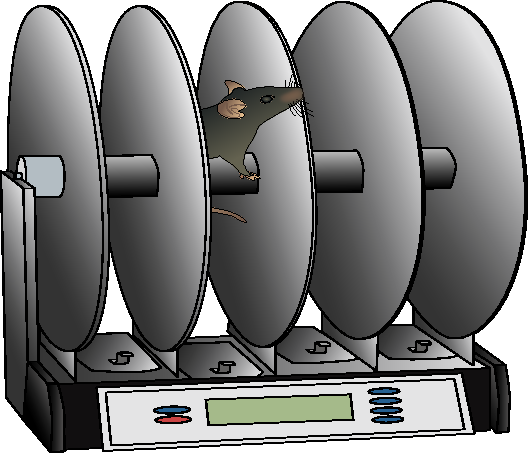
\includegraphics[width=0.5\linewidth]{figuras/expertos/experimento/rotarod.pdf}
    \caption{ Esquema del aparato rotarod.}
    \label{fig:rotarod}
\end{figure}

Cabe mencionar que cada prueba de \textit{rotarod} se lleva a cabo con un único ratón por vez sobre el cilindro, a pesar de que el aparato esté diseñado para albergar a más de un ratón simultáneamente. Esto se debe a que la presencia de múltiples ratones sobre el cilindro influye en sus comportamientos individuales.

Con el objetivo de correlacionar la actividad neuronal con el comportamiento (Capítulo \ref{cha:neuro}), los animales expertos analizados en este proyecto habían sido anteriormente inyectados en la región locomotora del mesencéfalo (MLR) con un virus que expresa canalrodopsina (ChR) sólo en neuronas glutamatérgicas. Se trata de un virus Cre-dependiente inyectado en un ratón transgénico que expresa Cre solamente en neuronas glutamatérgicas. Estos animales fueron también implantados con electrodos, para el registro de la actividad eléctrica en el MLR, y una fibra óptica, que permite la administración de luz para la activación de la ChR. De esta manera, se pretende lograr la identificación de la actividad registrada originada por neuronas glutamatérgicas a partir de su respuesta rápida y fiable a la luz. Cabe aclarar que ninguna de las neuronas registradas fueron positivamente identificadas como glutamatérgicas \cite{costa_motor_learning,luft_motor_learning,cardin_optogenetic}.

Una vez entrenados, los animales que denominaremos ``expertos'' en la tarea \textit{rotarod} fueron filmados mientras realizaban la tarea motora y se registró en simultáneo su actividad eléctrica en el MLR.

\section{Análisis de video}\label{sec:videos}

En esta parte del trabajo se analizaron los videos de los ratones expertos, adquiridos durante la realización de pruebas \textit{rotarod}. En estos videos se capturaron los movimientos de la parte posterior de los ratones. A partir de estos videos se extrajeron las posiciones $x$ e $y$ de las extremidades posteriores y de la cola del ratón, en función del tiempo, a una frecuencia de muestreo de 100 Hz. Para ello se utilizó \textit{DeepLabCut}, una herramienta \textit{open-source} que estima la posición de marcadores digitales definidos por el usuario. \textit{DeepLabCut} permite la estimación de poses animales basado en técnicas de transferencia de aprendizaje (\textit{transfer learning}) con redes neuronales artificiales profundas (\textit{deep neural networks}) y puede alcanzar un rendimiento equivalente al humano luego de haber entrenado la red con pocos fotogramas (\textit{frames}) de ejemplo (típicamente 50-200 \textit{frames}) \cite{mathis_deeplabcut}. Cabe mencionar que en esta parte del trabajo se contó con un total de 59 videos, provenientes de $N_{\mathrm{ratones}} = 3$ ratones diferentes sometidos al menos tres veces por día a pruebas \textit{rotarod}, durante un promedio de 6 días por ratón. En total, el cuerpo de videos adquiridos comprende alrededor de $N \sim 1$ millón de fotogramas para analizar.

La Figura \ref{fig:positions_panel}a muestra un fotograma típico de video analizado. En él, se marcaron las posiciones extraídas para las patas traseras y la base de la cola (con círculos en la figura). Además para cada fotograma se extrajeron las posiciones de las cuatro esquinas del cilindro rotarod. Esto se hizo a modo de calibración ya que se sabe que el ancho del cilindro es de 5.7 cm, permitiéndonos convertir los valores de las posiciones desde píxeles a centímetros. En la práctica, para cada \textit{trial rotarod} capturado en video, se calculó la mediana de la distancia entre las dos esquinas inferiores del cilindro rotarod en píxeles de forma tal de evitar la influencia de valores extremos. Esto sucede cuando un marcador digital es ocultado parcial o totalmente en el video (por ej., si el ratón oculta con su cuerpo a una de las esquinas del cilindro) y como consecuencia, el programa \textit{DeepLabCut} pierde precisión en la determinación de la posición del marcador ocultado. 

La Fig. \ref{fig:positions_panel}b muestra la evolución temporal típica de las componentes verticales de las posiciones de los marcadores de las patas traseras y de la base de la cola, en un intervalo de tiempo de 10 s luego de 10 s de comenzada la prueba de \textit{rotarod}. Pueden observarse patrones periódicos de movimiento en los diferentes marcadores y puede notarse que estos patrones de movimiento son asimétricos en el tiempo. También pueden observarse diferentes desfasajes en los movimientos de los marcadores, como así también diferentes grados de sincronización en el movimiento. En particular se observan de manera clara las instancias de movimiento voluntario (activo) e involuntario (pasivo) de las patas del ratón. Por un lado, junto a la serie temporal de la pata derecha en la Figura \ref{fig:positions_panel}b se indica con una flecha en línea continua negra el momento en el que el ratón da un paso con la pata derecha, levantándola bruscamente y desplazándose activamente hacia la parte superior del cilindro. Por otro lado, la flecha en línea discontinua negra indica el movimiento pasivo de deriva debido a la rotación del cilindro.

\begin{figure}[!htbp]
    \centering
    \begin{subfigure}{.35\textwidth}
        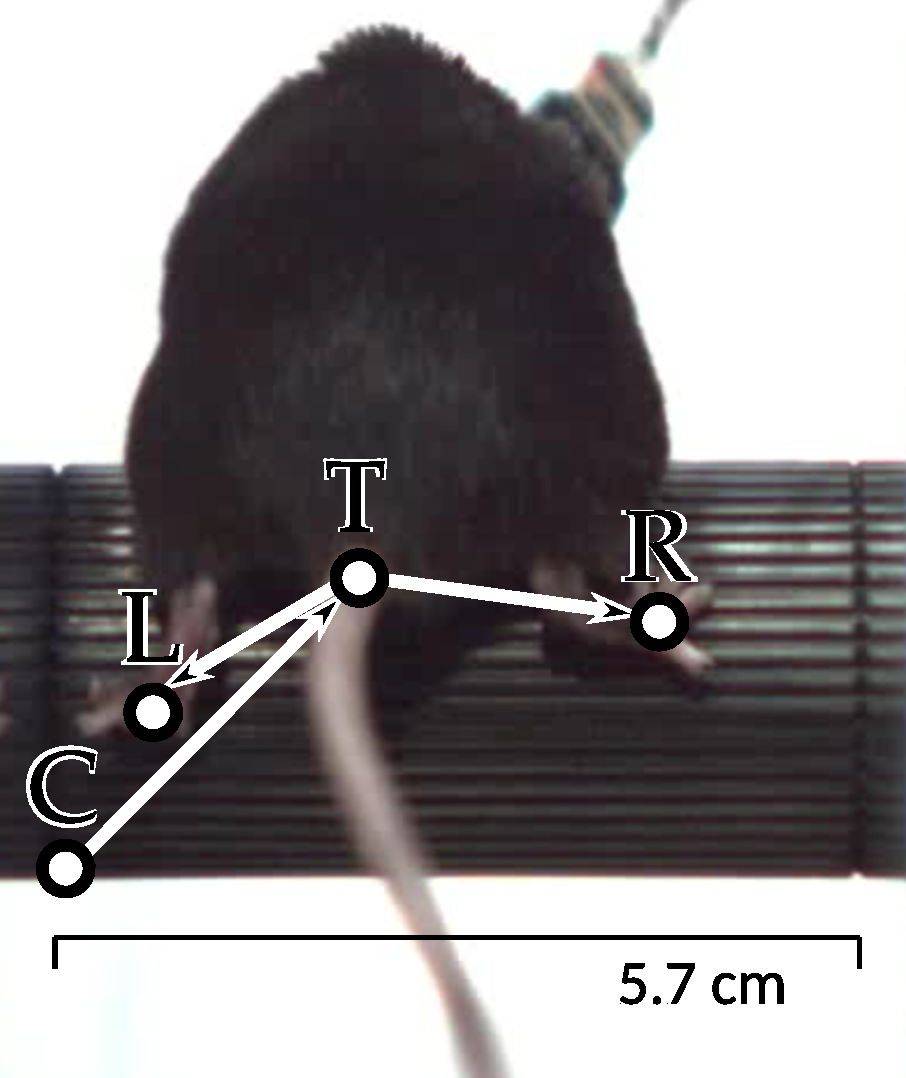
\includegraphics[width=1\linewidth]{figuras/expertos/videos/frame.pdf}
        \caption{}
    \end{subfigure}
    \begin{subfigure}{.64\textwidth}
        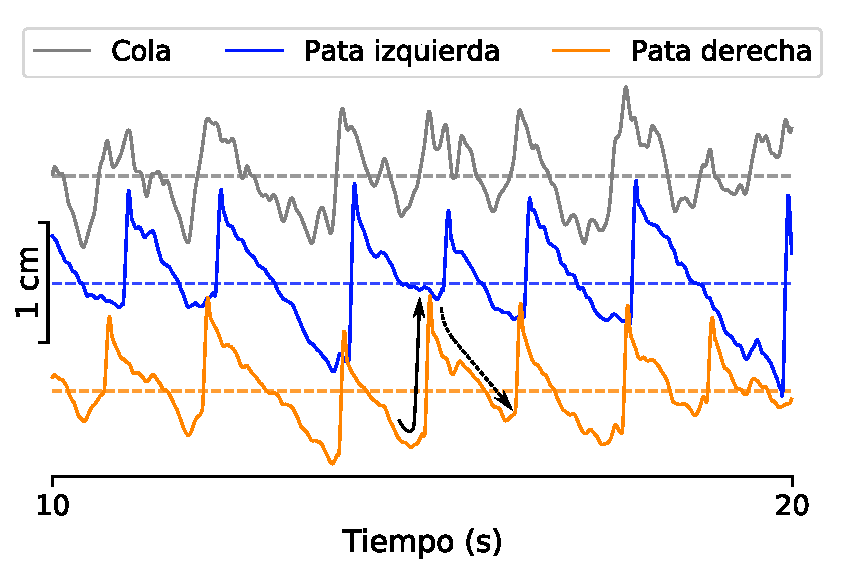
\includegraphics[width=1\linewidth]{figuras/expertos/videos/positions.pdf}
        \caption{}
    \end{subfigure}
    \caption{Caracterización de las posiciones de partes del cuerpo del ratón en función del tiempo. (a) Fotograma típico con las posiciones de los marcadores de la base de la cola y de las patas traseras (indicados por círculos). A partir de estas posiciones se calculan posiciones relativas (indicadas por flechas). (b) Serie temporal típica que muestra el movimiento sobre el eje vertical de los marcadores de la base de la cola y de las patas traseras (línea continua) y sus valores promedio en este intervalo de tiempo (línea discontinua). Con fines de visualización, los valores promedio de las series temporales se fijaron a 1 cm entre sí. Se marcó una instancia de movimiento activo (flecha en línea continua negra) y de movimiento pasivo (flecha en línea discontinua negra). }
\label{fig:positions_panel}
\end{figure}

Finalmente, debemos aclarar que se trabajó con posiciones relativas. Denotemos con $\vb{T}_i$ (\textit{tail}), $\vb{L}_i$ (\textit{left}), $\vb{R}_i$ (\textit{right}) y $\vb{C}_i$ (\textit{corner}) a las posiciones en el plano del fotograma $i$ de los marcadores de la base de la cola, de las patas izquierda y derecha y de la esquina inferior izquierda del cilindro \textit{rotarod}, respectivamente. A partir de estas, se calcularon las posiciones relativas $\widetilde{\vb{C}}_i - \vb{T}_i$, $\vb{T}_i - \vb{L}_i$ y $\vb{T}_i - \vb{R}_i$. Es decir, que describiremos el estado del ratón observado en el fotograma $i$-ésimo con estos 3 vectores bidimensionales, los cuales representan posiciones relativas entre marcadores. Así, construimos un vector de estado $\vb{x}_i$, para cada fotograma $i$ de video analizado, de la forma:
\begin{equation}
    \vb{x}_i = \mqty[\widetilde{\vb{C}}_i - \vb{T}_i\\ \vb{T}_i - \vb{L}_i\\ \vb{T}_i - \vb{R}_i],
\end{equation}
donde $\widetilde{\vb{C}}_i$ es la mediana de $\vb{C}_i$ para cada prueba \textit{rotarod} diferente (utilizamos su mediana pues la posición de la esquina del cilindro \textit{rotarod} es constante en cada prueba pero varía entre días sucesivos). De esta manera el vector de estado $\vb{x}_i$ tiene 6 componentes (pues está compuesto por 3 vectores bidimensionales) y existe una relación de correspondencia entre el estado en el fotograma $i$ con su evolución temporal a tiempo $t$
\begin{equation}
    \vb{x}_i \equiv \vb{x}(t).
\end{equation}

Con el objetivo de reducir el ruido asociado a la detección exacta de cada marcador, las posiciones de los marcadores $\vb{T}_i$, $\vb{L}_i$, $\vb{R}_i$ y $\vb{C}_i$ se suavizaron utilizando un filtro de Savitzky–Golay \cite{sav_gol} de ajuste polinomial de grado 3, con un ancho de ventana de 5 \textit{frames} de video. Para ello se utilizó la implementación en Python del filtro provista en el paquete de análisis de señales \texttt{scipy.signal}.

\section{Algoritmo t-SNE}\label{sec:tsne}

\subsection{Introducción y formalismo}\label{subsec:tsne_elementos}

Habiendo extraído estos vectores de estado $\vb{x}_i$ para cada fotograma $i$ de video analizado podemos buscar alguna manera de visualizarlos que nos ayude a dilucidar su estructura subyacente. Para ello, utilizaremos el algoritmo t-SNE, la cual es una herramienta popular en la comunidad bioinformática, principalmente para la visualización de datos de dimensión alta. El objetivo principal de esta transformada es reducir la dimensión de un conjunto de datos preservando su estructura local.

La transformada t-SNE produce un mapeo uno a uno entre dos espacios: uno de dimensión alta y otro de dimensión baja (generalmente de 1 a 3 dimensiones). Este espacio de dimensión alta es el espacio de entrada (\textit{input space}) o espacio de \textit{features} de la transformada t-SNE, y denotaremos al conjunto de vectores pertenecientes a este espacio como $\{\vb{x}_i|i= 1,\dots, N\}$, siendo $N$ es el número total de puntos. El espacio de dimensión baja, al que se quiere reducir nuestro conjunto de datos, es el espacio de salida (\textit{output space}) de la transformada o espacio de \textit{outcomes}. Denotaremos a este conjunto de vectores como $\{\vb{y}_i|i= 1,\dots, N\}$. Llamaremos a la imagen de la trasformada t-SNE, o sea al conjunto de puntos $\{\vb{y}_i\}$, como mapa de comportamientos de los ratones o etograma. La Tabla \ref{tab:tsne} detalla los elementos básicos y la notación que se utilizará para la descripción de la transformada t-SNE.

\begin{table}[!htbp]
\centering
\begin{tabular}{l|cc}
\textbf{Espacio} & \textbf{Entrada} (\textit{features}) & \textbf{Salida} (\textit{outcomes}) \\ \hline
Dimensión & Alta & Baja \\
Vector $i$-ésimo & $\vb{x}_i$ & $\vb{y}_i$ \\
Distancia & $d$, arbitraria & $||\cdot||$, usualmente $L_2$ \\
Similaridad (probabilidades) & $p_{ij}$ ($P$) & $q_{ij}$ ($Q$) \\
\textit{Kernel} & Gaussiano & t de Student
\end{tabular}
\caption{Elementos básicos de la transformada t-SNE y notación utilizada. Comparación entre los espacios de entrada y de salida.}
\label{tab:tsne}
\end{table}

La técnica t-SNE (\textit{t-Distributed Stochastic Neighbor Embedding}), introducida por van der Maaten y Hinton en 2008 \cite{vdm_tsne}, es la sucesora del algoritmo SNE (\textit{Stochastic Neighbor Embedding}) el cual fue originalmente desarrollado por Hinton y Rosweis en 2002 \cite{hinton_sne}. La transformada t-SNE consiste en mapear puntos similares en el espacio de entrada en puntos cercanos en el espacio de salida, preservando en el proceso la estructura local del conjunto de datos. Para ello es necesario definir métricas en el espacio de entrada y en el de salida. Usualmente las implementaciones de t-SNE permiten definir una métrica generalizada, o una manera de medir distancia arbitraria, $d$ en el espacio de entrada, mientras que convencionalmente se utiliza norma euclídea $L_2$ en el espacio de salida.

En nuestro caso, utilizamos en el espacio de entrada a la distancia coseno. Esta distancia se utiliza frecuentemente para analizar conjuntos de datos dispersos de dimensión alta en procesamiento de lenguaje natural (NLP, \textit{Natural Language Processing}), es independiente de la magnitud de los vectores y mide las orientaciones relativas de dos vectores en el espacio \cite{sidorov}.

\subsection{Cálculo de similaridades}\label{subsec:tsne_similaridad}

A partir de estas distancias, pueden definirse similaridades entre pares de puntos del espacio de entrada, utilizando un \textit{kernel} gaussiano, de la siguiente manera
\begin{equation}
    p_{j|i} = \frac{1}{\mathcal{Z}_i} \exp{\left( -\frac{d(\vb{x}_{i}, \vb{x}_{j})^2}{2\sigma_i^2} \right)},
\end{equation}
donde la función de partición $\mathcal{Z}_i$ se calcula como
\begin{equation}
    \mathcal{Z}_i = \sum_{k\neq i}\exp{\left( -\frac{d(\vb{x}_{i}, \vb{x}_{k})^2}{2\sigma_i^2} \right)}.
\end{equation}

De esta manera, la similaridad del punto $\vb{x}_j$, respecto del punto $\vb{x}_i$, es la probabilidad condicional $p_{j|i}$ de que el punto $\vb{x}_i$ elija al punto $\vb{x}_j$ como un vecino cercano. Esto sería si se eligieran vecinos cercanos en proporción a su densidad de probabilidad con una distribución gaussiana de distancias centradas en $\vb{x}_i$ \cite{vdm_tsne}. Fijamos $p_{i|i} = 0$, debido a que sólo nos interesa modelar similaridad entre pares de puntos diferentes. Estas $p_{j|i}$ también pueden interpretarse como la probabilidad de que ocurra una transición desde el estado $\vb{x}_i$ en el fotograma $i$ hacia un estado $\vb{x}_j$ en el fotograma siguiente $i+1$. Esto es así pues esperamos que para fotogramas consecutivos, el estado $\vb{x}$ varíe continuamente, pues su movimiento también es continuo. La introducción de estas probabilidades $p_{j|i}$ es lo que le da el nombre de ``estocástico'' (\textit{stochastic}) al algoritmo t-SNE y el hecho de que estas probabilidades sean de transición entre vecinos cercanos es también lo que le da la parte de ``\textit{neighbor}'' a su nombre.

Por último, estas similaridades se simetrizan de manera que sean equivalentes sin importar el orden en que se tomen los puntos del par $(\vb{x}_{i}, \vb{x}_{j})$
\begin{equation}
    p_{ij} = \frac{p_{j|i}+p_{i|j}}{2N},
\end{equation}
donde $N$ es el número total de puntos en el espacio de entrada. Este paso de simetrización fue introducido por primera vez en una variante de SNE conocido como SSNE (\textit{Symmetric Stochastic Neighbor Embedding}) \cite{yang_ssne}. Note además que $p_{ii} = 0$ y que $\sum_{i,j} p_{ij} = 1$, por lo que $p_{ij}$ resulta una distribución de probabilidad válida sobre el conjunto de todos los pares posibles de puntos $(\vb{x}_i, \vb{x}_j)$ \cite{kobak_art}. Simetrizar las probabilidades hace que no nos importe el orden de los fotogramas en los que estudiamos las transiciones.

La desviación estándar $\sigma_i$ del \textit{kernel} gaussiano se calcula para cada punto $\vb{x}_i$ del espacio de entrada de manera de mantener constante un parámetro predefinido $\mathcal{P}$, generalmente fijado en $\mathcal{P} = 30$, denominado perplejidad (\textit{perplexity})
\begin{align}
    \mathcal{P}_i &= \exp{H_i}\\
    &= \mathcal{P} \text{ (constante)},
\end{align}
siendo $H_i$ la entropía de Shannon de la distribución de probabilidad condicional $p_{j|i}$ de \textit{kernel} gaussiano definida anteriormente
\begin{equation}
    H_i = -\sum_{j} p_{j|i} \ln p_{j|i}.
\end{equation}

El parámetro de perplejidad $\mathcal{P}$ está relacionado con ${}^{q}D_i$, el índice de diversidad generalizado de orden $q$ (\textit{generalized diversity index}) \cite{jost_diversity, shannon_communication}, definido como
\begin{equation}
    ^{q}D_i = \left(\sum_{j} p_{j|i} \right)^{1/(1-q)},
\end{equation}
el cual, en el límite cuando $q\rightarrow 1$ equivale a la perplejidad
\begin{align}
    {}^{1}D_i &= \lim_{q \to 1} {}^{q}D_i\\
    &= \mathcal{P}_i.
\end{align}
Podemos pensar que la perplejidad es el número de vecinos más cercanos a los que transiciona el estado $\vb{x}_i$ del ratón. Aumentar (o reducir) este parámetro aumentará (o reducirá) entonces la cantidad total de vecinos que serán más relevantes para nuestras transiciones entre fotogramas. Además, usar una perplejidad demasiado baja nos daría una descripción miope de las transiciones posibles desde el estado $\vb{x}_i$ del ratón (podría sesgar nuestro mapa t-SNE), mientras que usar una perplejidad demasiado alta incluiría demasiados vecinos como cercanos. Esto último podría aumentar la variabilidad del mapa t-SNE, pero más grave para nuestros fines prácticos es que aumentaría mucho la complejidad de cómputo de del algoritmo t-SNE.

El número ${}^{q}D_i$ se conoce también como número efectivo de especies, y está definido en este caso en torno al punto $\vb{x}_i$. El número ${}^{q}D_i$ es una medida de la cantidad de puntos $\vb{x}_j$ (con $j \neq i$) que son similares a $\vb{x}_i$. Esto es, está relacionado con el concepto de vecinos cercanos al estado $\vb{x}_i$.

Existe un motivo por el cual la desviación estándar $\sigma_i$ se selecciona de manera tal que la perplejidad $\mathcal{P}_i$ se mantenga constante para cada punto $\vb{x}_i$ del espacio de entrada. Pues así se permite que el ancho del \textit{kernel} gaussiano $\sigma_i$ se adapte a las condiciones locales del conjunto de datos. Esto es, en regiones de densidad alta (baja) del conjunto de datos se utilizan valores más pequeños (grandes) de $\sigma_i$. Note además que la entropía $H_i$ aumenta al aumentar $\sigma_i$ \cite{vdm_tsne}. Esto es en parte lo que asegura que el mapa t-SNE preserve la estructura local de nuestro conjunto de datos.

Por otro lado, y de manera similar a como hicimos en el espacio de entrada, se definen similaridades en el espacio de salida de la forma
\begin{equation}
    q_{ij} = \frac{1}{\mathcal{Z}} \frac{1}{ 1 + ||\vb{y}_i - \vb{y}_j||^2 },
\end{equation}
donde la función de partición $\mathcal{Z}$ se calcula como
\begin{equation}
    \mathcal{Z} = \sum_{k} \sum_{l\neq k} \frac{1}{1+||\vb{y}_k-\vb{y}_l||^2}.
\end{equation}

De esta manera, las similaridades en el espacio de salida se calculan utilizando un \textit{kernel} de Cauchy (t de Student con grado de libertad $\nu = 1$). El objectivo del mapa t-SNE es que estas probabilidades $q_{ij}$ reflejan de la manera más fiel posible a las probabilidades $p_{ij}$ de nuestros datos. Esta es la clave para que el algoritmo t-SNE sea capaz de brindar una representación en un espacio, de por ejemplo 2 dimensiones, de un conjunto de datos de dimensión mayor, por ejemplo en nuestro caso de 6 dimensiones. Y esto es a lo que nos referimos cuando decimos que t-SNE preserva la estructura local de nuestros datos.

Ahora, un poco más de historia. Originalmente, el algoritmo SNE utilizaba un \textit{kernel} gaussiano para calcular las similaridades en el espacio de salida. Esta era la principal causa del llamado problema de hacinamiento (\textit{crowding problem}) \cite{hinton_sne, vdm_tsne}. Este problema consistía en una aglomeración de puntos en el centro del mapa, dificultando la visualización de diferentes \textit{clusters} de datos. Una de las primeras instancias para solucionar el problema fue la implementación de un \textit{kernel} con colas pesadas uniformes, técnica que se denominó UNI-SNE (haciendo alusión a la incorporación de una distribución uniforme), la cual añadía un término constante en el cálculo de la distribución de probabilidad $q_{ij}$ \cite{cook_unisne}. Finalmente, prevaleció la implementación t-SNE que utilizamos actualmente, la cual utiliza un \textit{kernel} de distribución t de Student en el espacio de salida, y esta es una distribución de colas pesadas.

La implementación de t-SNE puede generalizarse utilizando \textit{kernels} t de Student con grados de libertad $\nu$ arbitrarios \cite{kobak_heavy_tail}. Esto nos permite obtener mapas t-SNE con \textit{clusters} mejor definidos. De esta manera, si se define un nuevo parámetro $\alpha$ tal que $\nu = 2\alpha - 1$, el \textit{kernel} adopta la forma
\begin{equation}
    q_{ij} = \frac{1}{\mathcal{Z}} \frac{1}{\left(1+||\vb{y}_i-\vb{y}_j||^2/\alpha\right)^\alpha},
\end{equation}
donde esta vez la función de partición $\mathcal{Z}$ se calcula como
\begin{equation}
    \mathcal{Z} = \sum_{k} \sum_{l\neq k} \frac{1}{ \left(1 + \frac{1}{\alpha}||\vb{y}_k - \vb{y}_l||^2 / \alpha \right)^\alpha}.
\end{equation}

Por último, fijamos $q_{ii} = 0$. Note que $\sum_{i,j} q_{ij} = 1$ por lo que $q_{ij}$ resulta, al igual que $p_{ij}$, una distribución de probabilidad válida sobre el conjunto de todos los pares de puntos, esta vez $(\vb{y}_i, \vb{y}_j)$. Definamos entonces como $P$ y $Q$ a los conjuntos de probabilidades $\{p_{ij}\}$ y $\{q_{ij}\}$ sobre todos los pares posibles $(i,j)$, respectivamente.

Ahora que hemos calculado estas probabilidades de transición $P$ y $Q$, ¿cómo hacemos para obligar a las probabilidades $Q$ a parecerse más a las probabilidades $P$? Esto se hace definiendo una función de costo, que penalice las diferencias entre $P$ y $Q$. De esta manera, minimizar la función de costo sería equivalente a obtener un mapa t-SNE en donde las probabilidades $Q$ mejor reflejan a las probabilidades $P$.

\subsection{Función de costo}\label{subsec:tsne_costo}

Como dijimos, el objetivo del algoritmo t-SNE es conseguir una representación de baja dimensión ($\{\vb{y}_i\}$) de nuestros datos ($\{\vb{x}_i\}$) que mejor conserve las similaridades entre pares de puntos. De esta manera, podemos capturar en el análisis el concepto de que el animal no se mueve instantáneamente de un extremo a otro del espacio, sino que hay una relación de proximidad entre puntos. Para este fin se utiliza la divergencia de Kullback-Leibler (KLD, \textit{Kullback-Leibler Divergence}) como función de costo. La KLD es una medida de qué tan parecidas son dos distribuciones de probabilidad y en nuestro caso coincide con la entropía cruzada de las distribuciones $P$ y $Q$ a menos de una constante \cite{vdm_tsne}. De esta manera, el proceso de optimización de un mapeo t-SNE consiste en minimizar la siguiente función de costo
\begin{align}
    \mathcal{L} &= D_{\mathrm{KL}}\left(P||Q\right)\\
    &= \sum_{i\neq j} p_{ij} \log_2\frac{p_{ij}}{q_{ij}}.
\end{align}

Por un lado, si las probabilidades $P$ y $Q$ son exactamente iguales, entonces la función de costo es cero (este es el mínimo valor que puede adquirir), por otro lado, si las probabilidades $P$ y $Q$ son muy diferentes, la función de costo puede adoptar un valor arbitrariamente grande. Además esta función de costo penaliza más fuertemente cuando fallamos en modelar probabilidades de transición $p_{ij}$ altas, que cuando fallamos en modelar $p_{ij}$ bajas. Esto permite que nuestro mapa t-SNE refleje mejor las características más salientes de nuestros datos.

La minimización de la función de costo se realiza mediante descenso por gradientes (\textit{gradient descent}). Dentro de la expresión del gradiente pueden identificarse dos términos
\begin{equation}
    \frac{1}{4}\frac{\partial\mathcal{L}}{\partial\vb{y}_i} = \underbrace{\varepsilon \sum_{j \neq i} p_{ij}  w_{ij}^{1/\alpha} \qty(\vb{y}_i - \vb{y}_j)}_{\substack{\text{Término atractivo}}} - \underbrace{\sum_{j \neq i} q_{ij}  w_{ij}^{1/\alpha} \qty(\vb{y}_i - \vb{y}_j),}_{\substack{\text{Término repulsivo}}}
    \label{eq:grad_tsne}
\end{equation}
donde se agrega al término atractivo un factor multiplicativo $\varepsilon$ denominado exageración (\textit{exaggeration}), cuyo valor por defecto es $\varepsilon = 1$ \cite{linderman_tsne} y definiendo además a $w_{ij}$ en la expresión (\ref{eq:grad_tsne}) como
\begin{equation}
    w_{ij} = \left( 1+||\vb{y}_i-\vb{y}_j||^2/\alpha \right)^{-\alpha}.
\end{equation}

Una manera de interpretar el gradiente de la función de costo es como si fueran sumas de fuerzas de ``resortes'' que unen a todos los pares de puntos $(\vb{y}_i, \vb{y}_j)$ del mapa t-SNE. Así, un punto $\vb{y}_i$ del mapa t-SNE sufre fuerzas que pueden ser tanto atractivas como repulsivas en las direcciones $\vb{y}_i - \vb{y}_j$. Siguiendo esta interpretación, optimizar el mapa t-SNE, que equivale a minimizar la función de costo, equivale también a encontrar el equilibrio de las fuerzas de todos estos resortes \cite{cook_unisne}.

Finalmente, las posiciones {$\vb{y}_i$} del mapeo t-SNE se actualizan, al final de una determinada iteración $n$, de acuerdo a la siguiente regla \cite{vdm_tsne, yang_ssne}
\begin{equation}
    \vb{y}_i^{(n+1)} = \vb{y}_i^{(n)} + \eta \frac{\partial\mathcal{L}}{\partial\vb{y}_{i}}\Big|_{\vb{y}_{i} = \vb{y}_{i}^{(n)}} + \beta^{(n)} \left( \vb{y}_{i}^{(n)} - \vb{y}_{i}^{(n-1)} \right),
\end{equation}
siendo $\eta$ la tasa de aprendizaje (\textit{learning rate}) y $\beta^{(n)}$ el \textit{momentum} en la iteración $n$.

Generalmente, las posiciones {$\vb{y}_i$} del mapeo t-SNE se inicializan como las primeras componentes principales (PCA, \textit{Principal Component Analysis}) del conjunto de datos {$\vb{x}_i$}. Luego, el proceso de optimización se repite usualmente alrededor de $n_{\mathrm{iter}} = 1000$ iteraciones. Originalmente, en la implementación SNE de Hinton, las posiciones {$\vb{y}_i$} se inicializaban de manera aleatoria \cite{hinton_sne}. Utilizar PCA para inicializar el mapa t-SNE tiene la ventaja de obtener mapas que son reproducibles, pues se elimina la aleatoriedad en su inicialización. Además, inicializar con PCA mejora la estructura global del mapa t-SNE, pues se basa en representar nuestro conjunto de datos a lo largo de las direcciones de mayor varianza del mismo, brindando una primera descripción ``a grandes rasgos'' \cite{kobak_art}.

Para adentrarse más en los detalles de implementación y para saber más sobre diferentes técnicas utilizadas en la optimización de los mapas t-SNE, por favor referirse a los Apéndices \ref{sec:tsne_aprox} y \ref{sec:tsne_optim}.

\subsection{Obtención del mapa de comportamientos}\label{subsec:tsne_aprox}

En este trabajo se utilizó la implementación en Python \texttt{openTSNE} \cite{policar_tsne} del algoritmo t-SNE. También existen implementaciones de paramétricas de t-SNE en \texttt{TensorFlow} y \texttt{Keras}, aunque la primera implementación de este tipo fue desarrollada en MatLab \cite{vdm_tsne}. La implementación \textit{benchmark} del algoritmo en Python es la de \texttt{scikit-learn} \cite{scikit-learn}. La implementación \texttt{openTSNE} nos brinda una gran flexibilidad en el control de los parámetros y del proceso de optimización. El Apéndice \ref{sec:tsne_param} brinda un resumen de los parámetros utilizados en nuestro mapa.

La Figura \ref{fig:tsne_black} muestra el mapa comportamientos o etograma obtenido al aplicar la transformada t-SNE sobre el conjunto de vectores de estado $\{\vb{x}_i\}$. Este mapa se construyó usando todos los fotogramas analizados correspondientes a los $N_{\mathrm{ratones}} = 3$ ratones observados. Recordemos que el vector de estado $\vb{x}_i$ contiene información sobre las posiciones relativas de algunas partes del cuerpo del ratón en el fotograma $i$-ésimo, durante la ejecución de la tarea motora \textit{rotarod} con aceleración. Por lo tanto, este mapa es una representación de las posiciones relativas de los ratones y de sus partes del cuerpo.

\begin{figure}[!htbp]
    \centering
    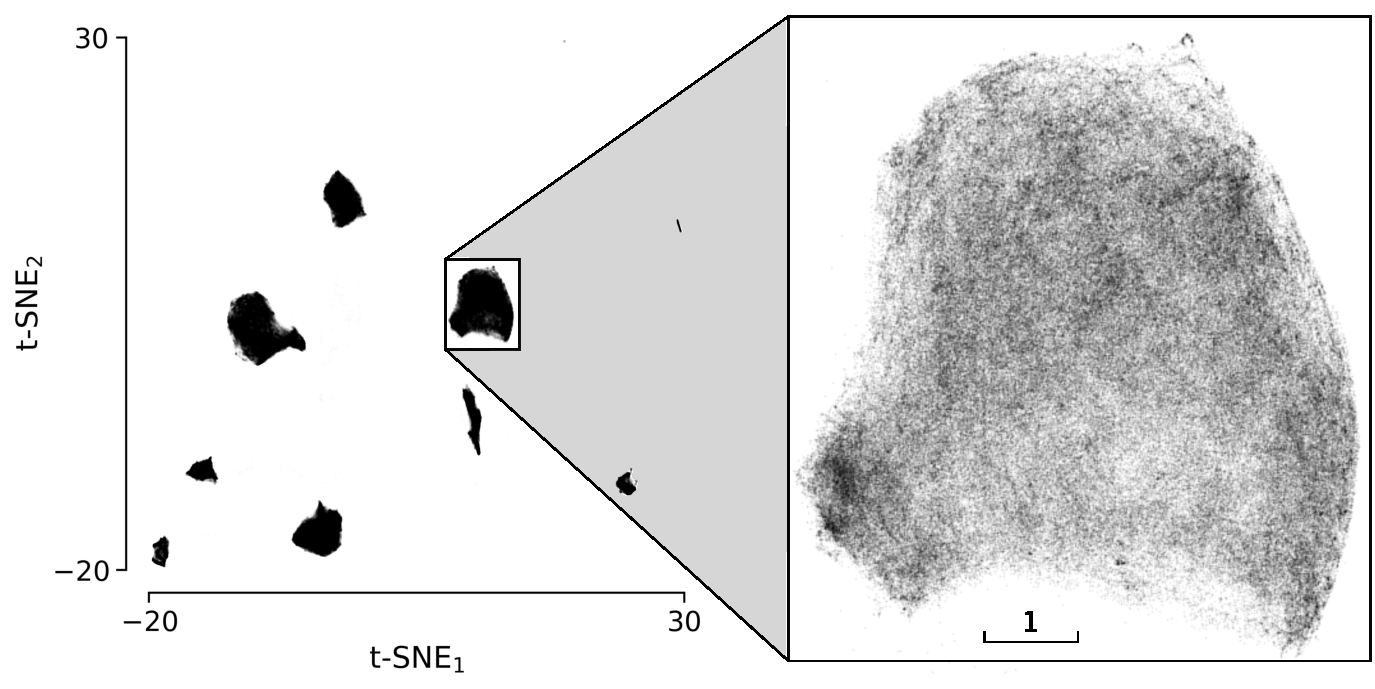
\includegraphics[width=\linewidth]{figuras/expertos/tsne/tsne_black.pdf}
    \caption{ Etograma obtenido a partir de la transformada t-SNE del conjunto de vectores de estado $\{\vb{x}_i\}$ de todos los \textit{frames} de video analizado. Estos vectores de estado representan las posiciones relativas de algunas partes del cuerpo de los ratones. Dentro del recuadro se muestra más en detalle los puntos de una región del etograma. }
    \label{fig:tsne_black}
\end{figure}

En el etograma de la Figura \ref{fig:tsne_black} puede observarse la aparición de \textit{clusters} de puntos. Cada punto $\vb{y}_i$ en el mapa t-SNE de la Figura \ref{fig:tsne_black} es la transformada de un vector de estado $\vb{x}_i$. Además, sabemos que la transformada t-SNE conserva la estructura local del conjunto de datos $\{\vb{x}_i\}$ y que puntos $\vb{y}_i$ cercanos en el mapa t-SNE se corresponden con vectores $\vb{x}_i$ similares. Entonces podríamos pensar que cada uno de los \textit{clusters} que se observan en el mapa t-SNE representan subconjuntos de vectores de estado $\{\vb{x}_i\}_l$ similares, donde $l$ es el número de clase o de pertencia al \textit{cluster} $l$-ésimo. Llamaremos $labels$ a estos números de clase o de pertenencia al \textit{cluster} $l$-ésimo. En la siguiente sección detallaremos el proceso de segmentación del etograma, mediante el cual asignaremos a cada punto del mapa t-SNE un $label$ determinado. Para ello utilizaremos la transformación divisoria (\textit{watershed}).

\section{Transformación \textit{watershed}}\label{sec:watershed}

Si bien el mapa t-SNE obtenido presenta \textit{clusters} muy bien definidos, quisimos segmentar estos \textit{clusters} de manera automática e independiente del usuario. Para ello utilizamos la transformación \textit{watershed}, que es un algoritmo de segmentación de imágenes en escala de grises. Una imagen en escala de grises puede pensarse como un relieve topográfico, donde el nivel de gris de cada píxel se interpreta como su altura en el mapa de relieve. Cuando se vuelca agua sobre un relieve topográfico, esta fluye a lo largo de diferentes caminos hasta finalmente llegar a un mínimo local de potencial. Intuitivamente, la divisoria de un relieve corresponde a los límites de las cuencas hidrográficas adyacentes. Esencialmente esta es la interpretación del funcionamiento de la transformación \textit{watershed} \cite{meyer_topographic, meyer_beucher_morphological}.

La transformación \textit{watershed} presenta una gran flexibilidad en cuanto al número total de regiones que se pueden segmentar en el plano, ya que dicho valor no requiere estar predeterminado. Además no representa una limitación en cuanto a complejidad computacional, ya que en nuestro caso se aplica directamente sobre la densidad de probabilidad de nuestro mapa t-SNE, y no sobre el conjunto de todos los puntos $\{\vb{y}_i\}$ del mapa.

La Figura \ref{fig:tsne_pdf}a muestra una estimación de densidad de probabilidad con \textit{kernel} gaussiano (KDE) de ancho de banda (\textit{bandwidth}) $\sigma=1$, para la distribución de puntos en el mapa t-SNE de la Figura \ref{fig:tsne_black}. La densidad de probabilidad se calculó utilizando el módulo \texttt{fastKDE} \cite{obrien_fastkde} implementado en Python, junto con un filtro de convolución gaussiano de la librería \texttt{scikit-image} \cite{scikit-image}. La implementación \texttt{fastKDE} aprovecha la transformada rápida de Fourier no uniforme (nuFFT), para conseguir una complejidad computacional $O(N)$, lo cual es muy eficiente para nuestros propósitos. La densidad de probabilidad se calculó sobre una cuadrícula con una resolución de $2049 \times 2049$ px$^2$. Esta resolución es más que suficiente para nuestra tarea de segmentación.

\begin{figure}[!htbp]
    \centering
    \begin{subfigure}{.49\textwidth}
        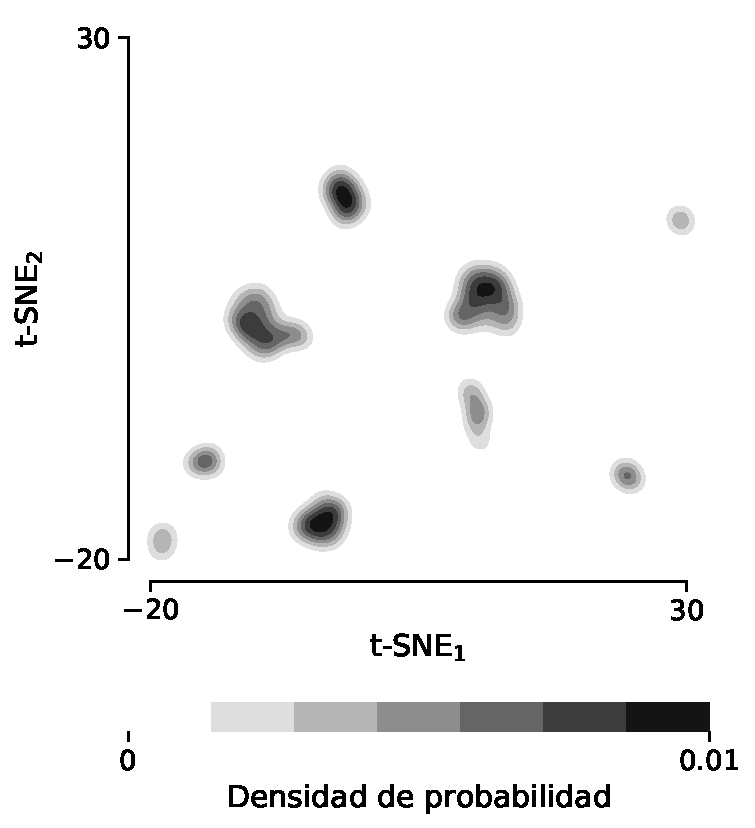
\includegraphics[width=1\textwidth]{figuras/expertos/watershed/relief_sig_tsne1.0_foot30_cut20.pdf}
        \caption{}
    \end{subfigure}
    \begin{subfigure}{.49\textwidth}
        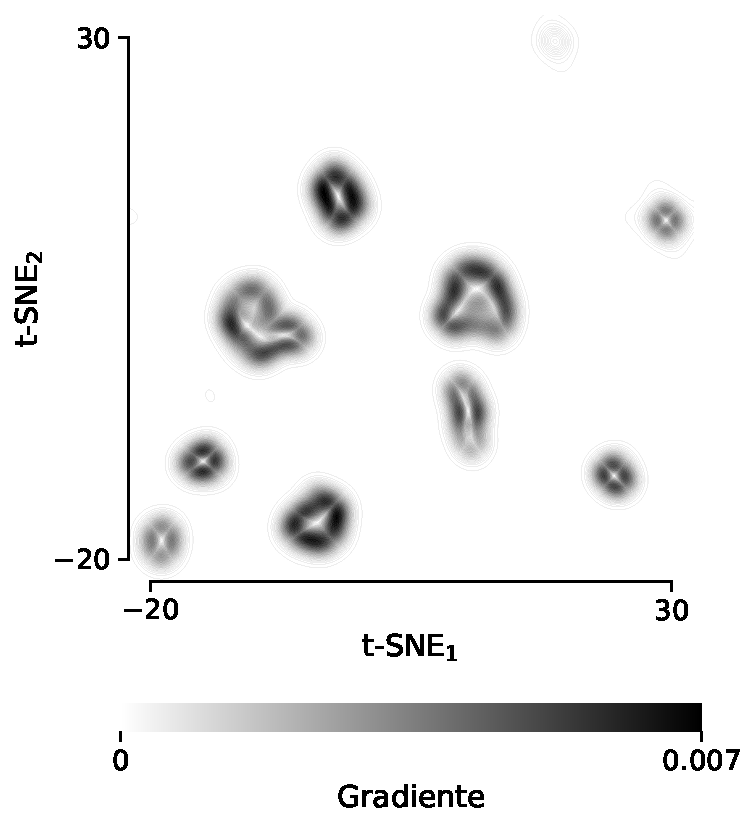
\includegraphics[width=1\textwidth]{figuras/expertos/watershed/gradient_sig_tsne1.0_foot30_cut20.pdf}
        \caption{}
    \end{subfigure}
    \caption{ Estimación de la distribución de densidad de probabilidad con \textit{kernel} gaussiano (KDE) de puntos del mapa t-SNE de la Figura \ref{fig:tsne_black}. (a) Superficies de nivel de la KDE. (b) Gradiente de la KDE.}
    \label{fig:tsne_pdf}
\end{figure}

La densidad de probabilidad que se muestra en la Figura \ref{fig:tsne_pdf}a presenta picos rodeados por amplios valles. En nuestro caso, nos interesa segmentar el mapa t-SNE en torno a estos picos de alta probabilidad y no en torno a las cuencas de baja probabilidad, pues lo que queremos es encerrar a los picos dentro de una única región. Por este motivo inicializamos la transformación \textit{watershed} utilizando un conjunto de máximos locales de la densidad de probabilidad. Por su parte, la Figura \ref{fig:tsne_pdf}b muestra el gradiente de la densidad de probabilidad de nuestro mapa t-SNE. La transformación \textit{watershed} encuentra regiones conexas en el mapa t-SNE, tales que si subimos a favor del gradiente de densidad de probabilidad dentro de una de estas regiones, llegamos a un mismo máximo local.

Cabe mencionar que antes de realizar la transformación \textit{watershed} se aplica un filtro de mediana usando una máscara de disco de radio de 2 px para reducir el ruido de la imagen de la densidad de probabilidad, y el resultado es el que se muestra en la Figura \ref{fig:tsne_pdf}a. Luego, se aplica un filtro de gradiente a la imagen, obteniéndose así la Figura \ref{fig:tsne_pdf}b. Este filtro de gradiente se aplicó también con una máscara de disco de 2 px de radio. De esta manera se obtiene la imagen que funcionará como guía para delimitar las fronteras entre las distintas regiones en la segmentación del mapa t-SNE.

Finalmente la Figura \ref{fig:tsne_labels} muestra el mapa de comportamientos segmentado en $N_{\mathrm{clases}} = 9$ regiones diferentes, y las fronteras entre regiones contiguas. Cada una de estas regiones encierra un \textit{cluster} bien definido e incluye algunos puntos fuera del \textit{cluster} principal a los cuales se les asigna una misma etiqueta de pertenencia de clase, es decir un \textit{label} único. Sobre la Figura \ref{fig:tsne_labels} se anotaron los números de \textit{label} asignados a cada región segmentada. Los números de \textit{label} se colocaron en la posición del centro de masa de cada región. Note que la región de \textit{label} número 8 es la única que encierra dos \textit{clusters} separados, aunque el centro de masa de esta región está ubicado encima de uno de ellos, por lo que el peso del \textit{cluster} más alejado es despreciable en comparación.

\begin{figure}[!htbp]
    \centering
    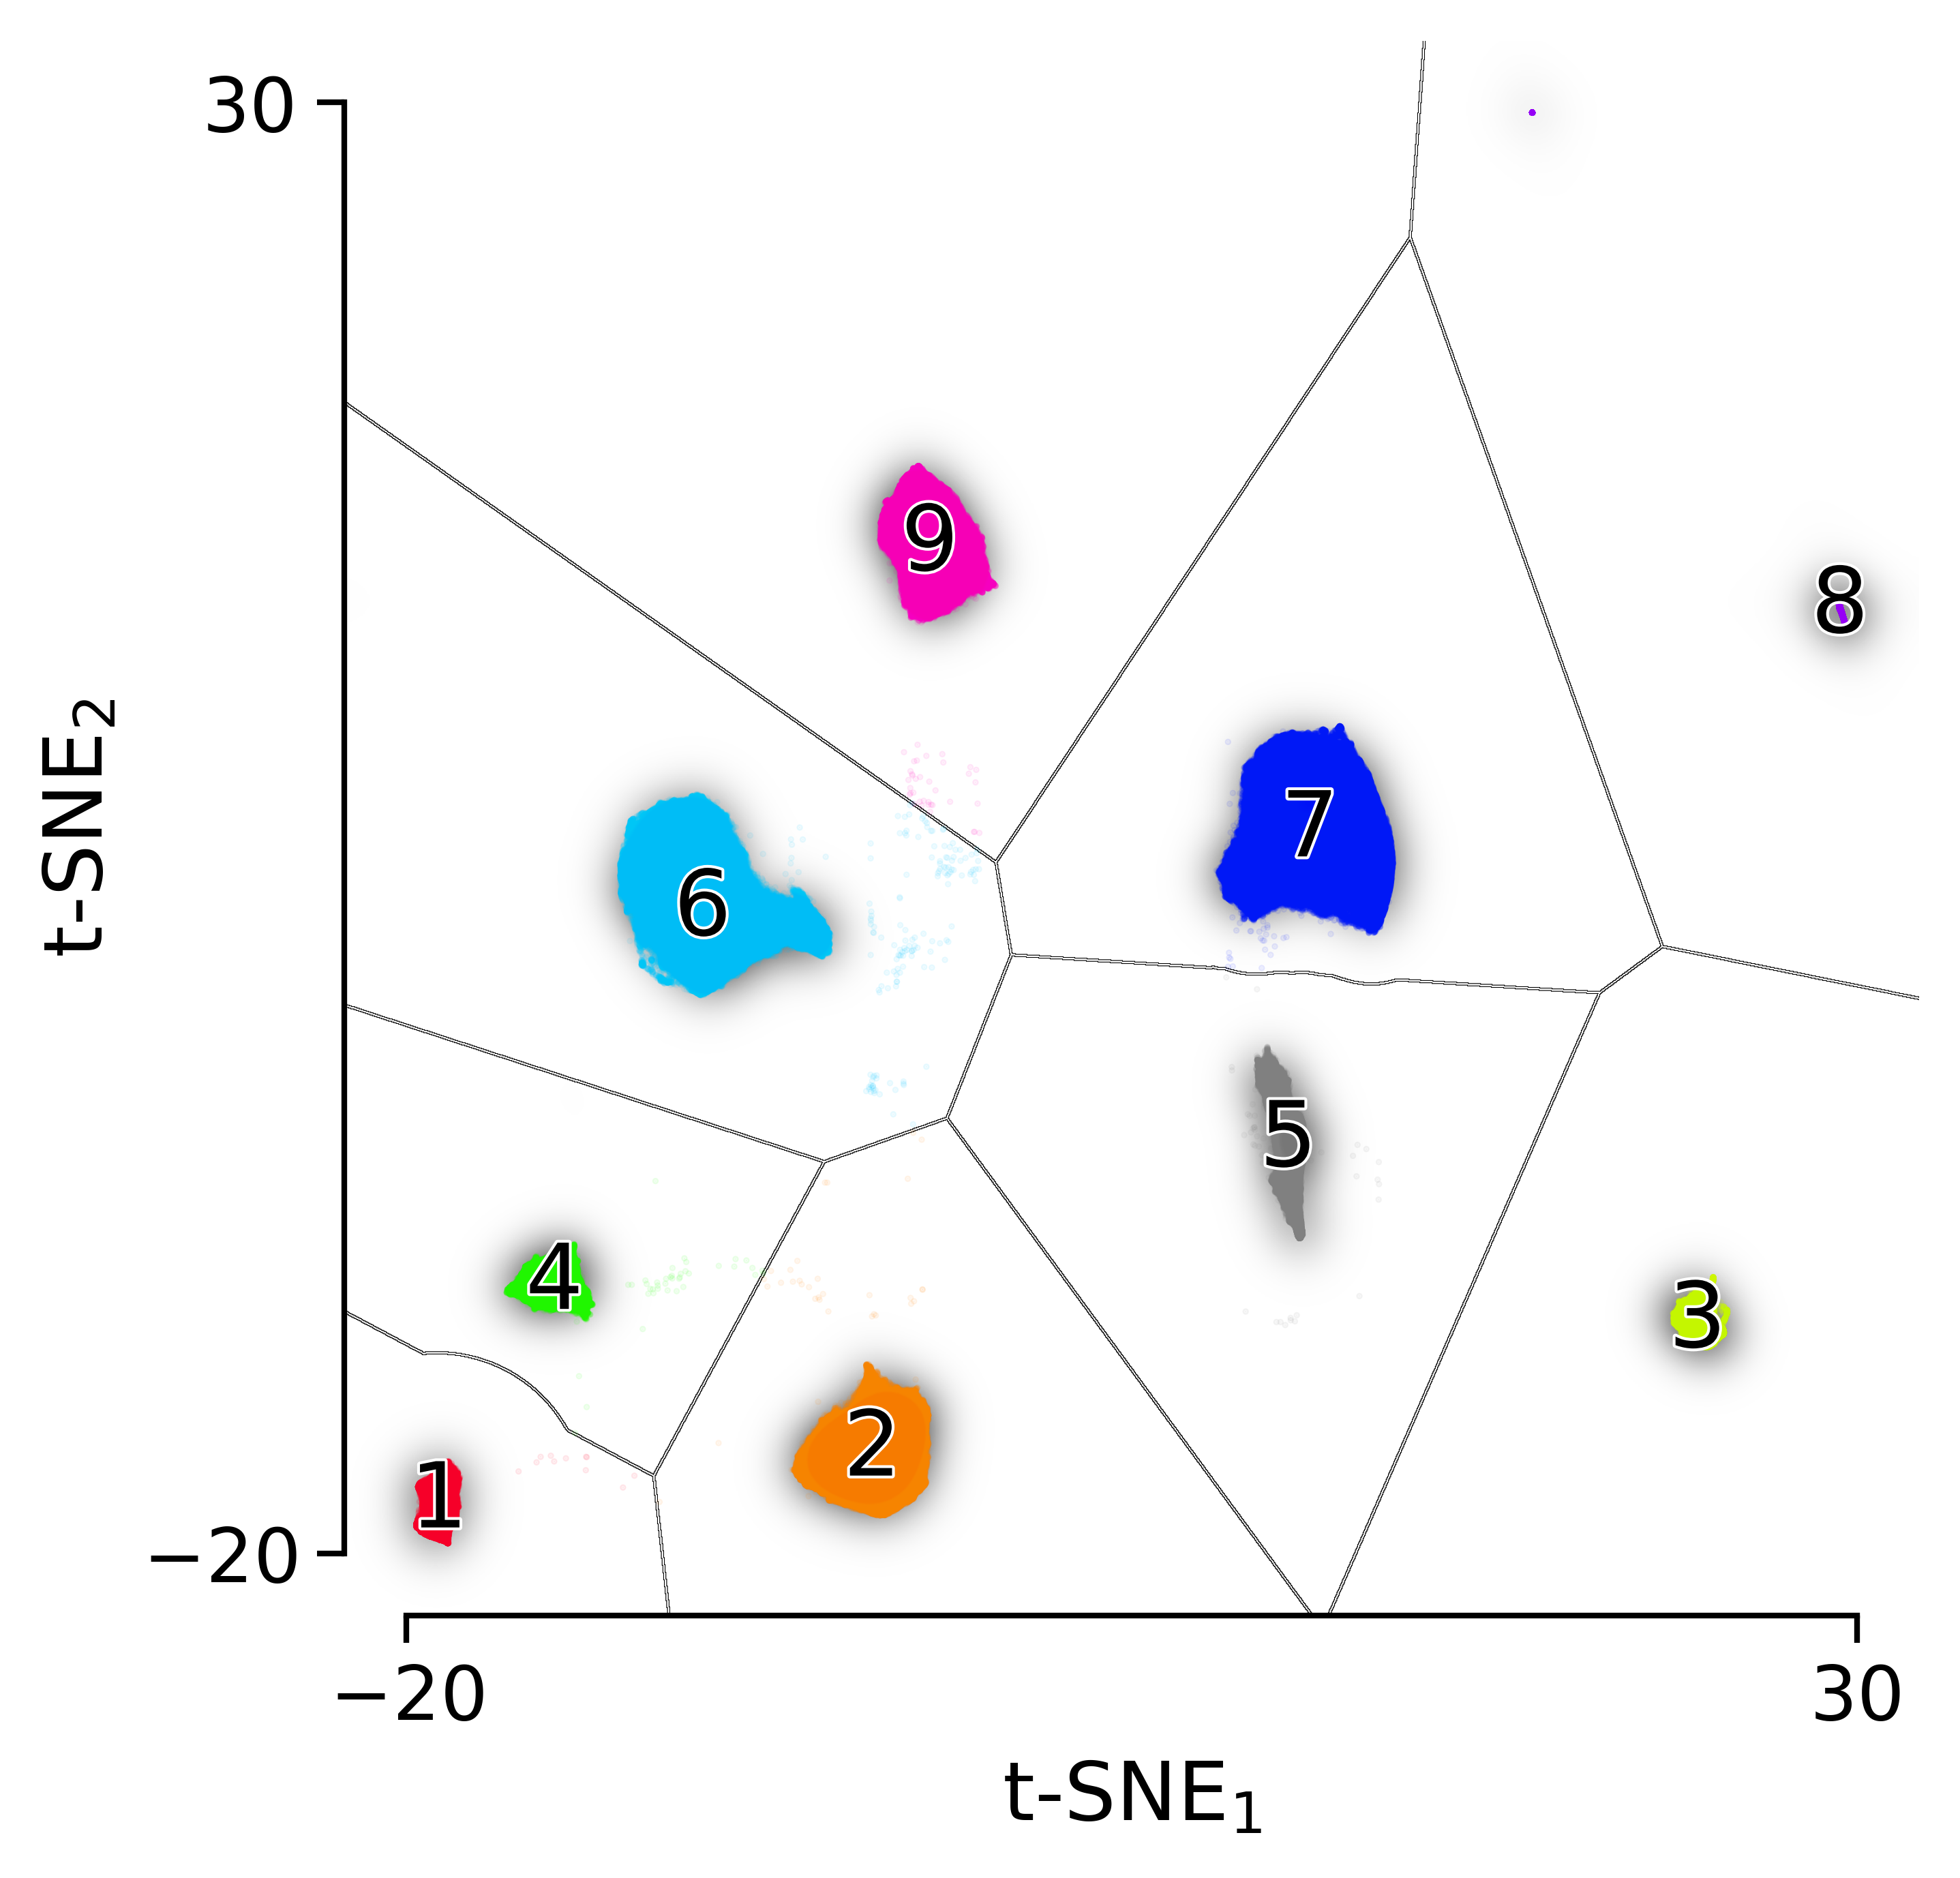
\includegraphics[width=1\linewidth]{figuras/expertos/labels/segmentation.png}
    \caption{Mapa de comportamientos obtenido a partir del conjunto de vectores de estado $\{\vb{x}_i\}$ de todos los fotogramas de video analizados. En este mapa t-SNE se anotaron los números de clase (\textit{labels}) asignados a cada región segmentada. Estas anotaciones se posicionaron encima de los centros de masa de cada región. Se marcaron las fronteras entre regiones contiguas. Los puntos están coloreados de acuerdo al \textit{label}.}
    \label{fig:tsne_labels}
\end{figure}

En el siguiente capítulo estudiaremos algunas propiedades del etograma obtenido a través del algoritmo t-SNE. También exploraremos e interpretaremos los \textit{labels} que resultaron de la segmentación mediante transformación \textit{watershed}.